\chapter{Implementazione}
\label{implementazione}
In questo capitolo vengono illustrati i dettagli implementativi riguardanti le realizzazioni hardware e software del sistema realizzato nell'ambito di questa tesi.

\section{Implementazione Hardware}
\label{impl_hardware}
In questa sottosezione verrà mostrato inizialmente uno schema con i componenti hardware utilizzati per realizzare il sistema ideato in sez.\ref{descrizioeDelLavoro}, per finire verranno illustrati i canali di comunicazione.
\subsection{Schema hardware del sistema}
Con riferimento alla rappresentazione astratta del sistema a moduli presentata nella sez.\ref{livello_moduli}, segue una il medesimo schema ad un livello meno astratto nel quale si mostrano le componenti hardware che costituiscono i due moduli App e microcontrollore.
\begin{sidewaysfigure}[htbp]
	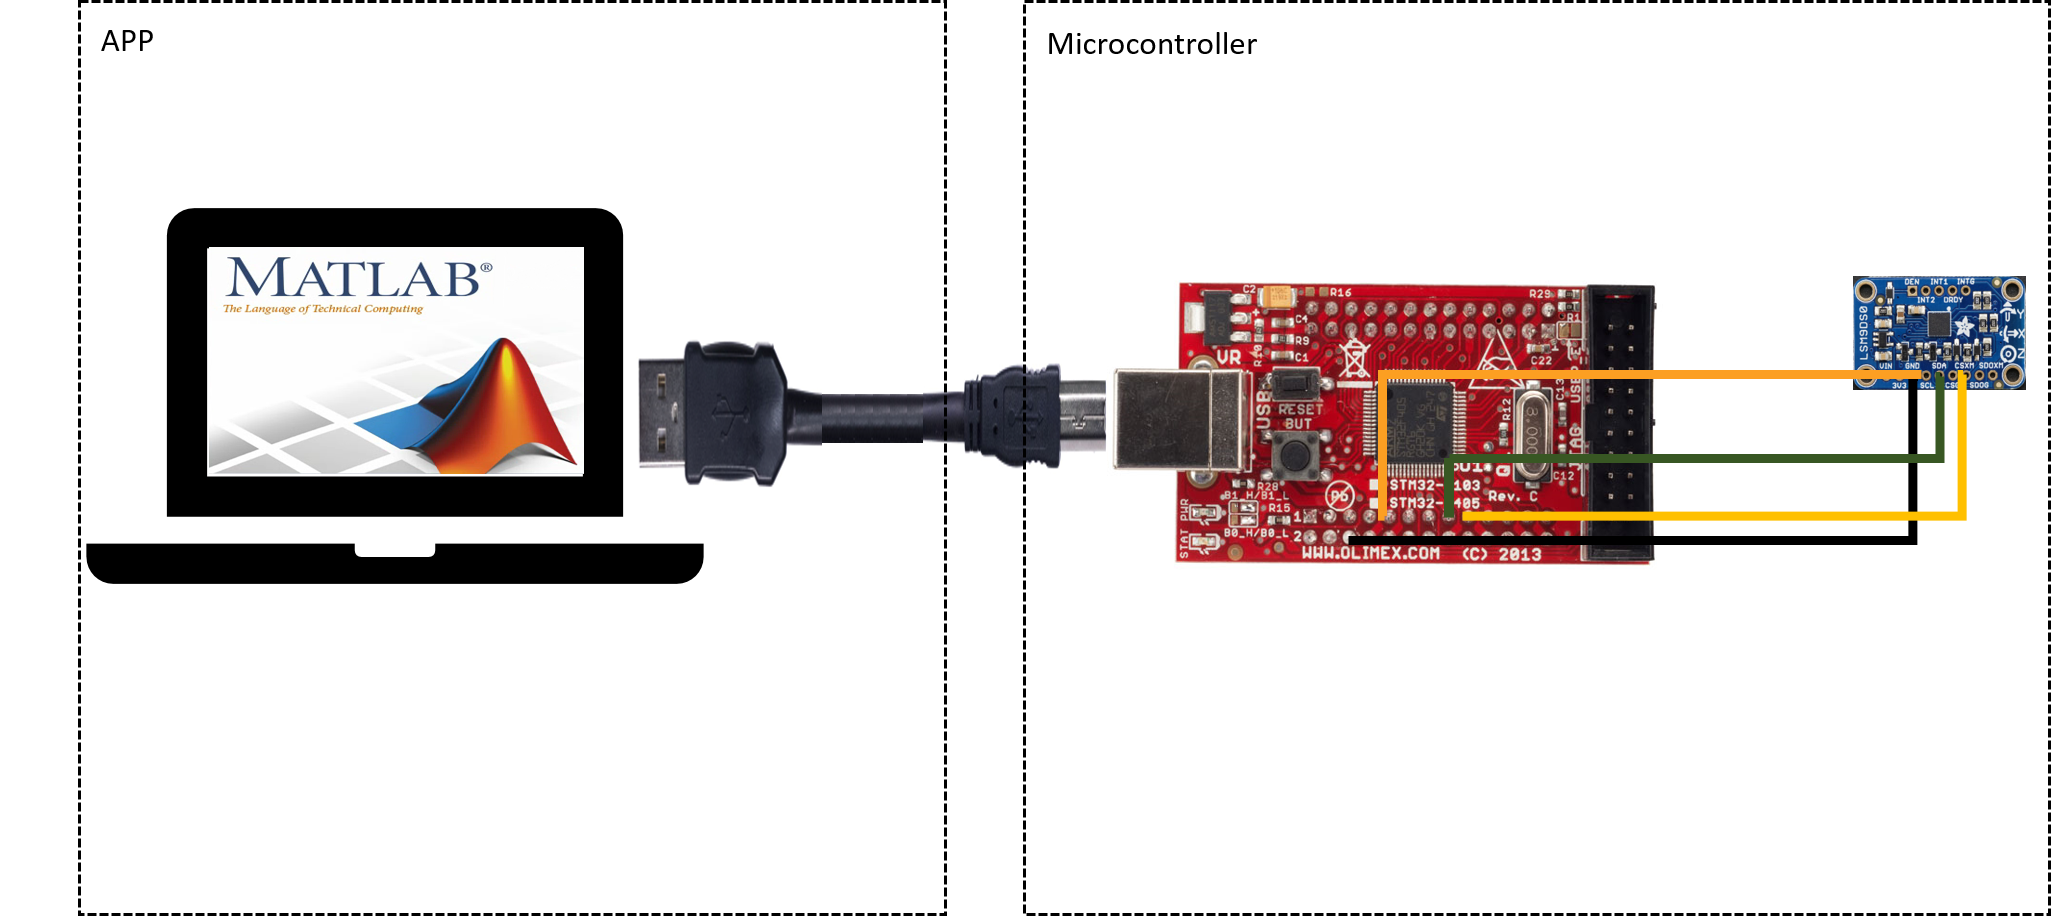
\includegraphics[width=\textwidth]{implementazione/schemaHardware.png}
	\caption{Schema hardware del sistema}
	\label{fig:schemaHardware}
\end{sidewaysfigure}
\newpage
Dove:
\begin{itemize}
	\item \textbf{Il modulo APP}: è composto da un'elaboratore nel quale si utilizzano i seguenti software
	\begin{itemize}
	\item \textit{RealTerm} per catturare in un file di log i dati inviati dal moduli microcontrollore
	\item \textit{Matlab} per testare l'algoritmo di \textit{Sensor Fusion} ed effettuare le varie analisi (sez.\ref{analisi})
	\end{itemize}
	\item \textbf{Il modulo Microcontrollore}: è composto da
	\begin{itemize}
		\item Una board Olimex con microcontrollore STM32F405 prodotto da \textit{STM}
		\item Un'unità di misura inerziale LSM9DS1 prodotta da \textit{STM}
	\end{itemize}
\end{itemize}
E' necessario spendere due parole a riguardo dell'implementazione del modulo APP mostrata in Fig.\ref{fig:schemaHardware}. \\
Relativamente al contesto applicativo individuato per questo sistema (sez.\ref{contesto}) l'applicativo Matlab e, più in generale, l'elaboratore non sono adatti alla realizzazione di un sistema IPS real-time. Tuttavia nel lavoro di questa tesi, questi vengono utilizzati al solo fine di comparare l'algoritmo di \textit{Sensor fusion} implementato (sez.\ref{sensor_fusion}) con quello eseguito all'interno del microcontrollore e di effettuare ulteriori analisi (sez.\ref{analisi}). Le fasi successive dello sviluppo di questo sistema, prevedono infatti lo studio della realizzazione ottima del modulo APP a partire dai risultati ottenuti dal lavoro di questa tesi.


\subsection{Canali di comunicazione}
In questa sezione verranno illustrati i canali di comunicazione (mostrati in Fig.\ref{fig:schemaHardware}) utilizzati per la trasmissione dei dati all'interno del sistema realizzato nell'ambito di questa tesi. Il primo paragrafo tratta il canale di comunicazione utilizzato tra il microcontrollore e l'unità di misura inerziale mentre nel secondo e ultimo paragrafo il canale di comunicazione utilizzato per trasmettere dati dal microcontrollore all'applicativo terminale sull'elaboratore.
\subsubsection{I2C}
\label{imp_i2c}
Per la comunicazione tra l' \textbf{IMU} e il \textbf{Microcontrollore}, si è utilizzato un canale di comunicazione seriale bifilare noto come \textit{Inter Integrated Circuit}, abbreviato \textbf{I2C}, come mostrato dalla seguente figura:
\begin{figure}[H]  
	\centering 
	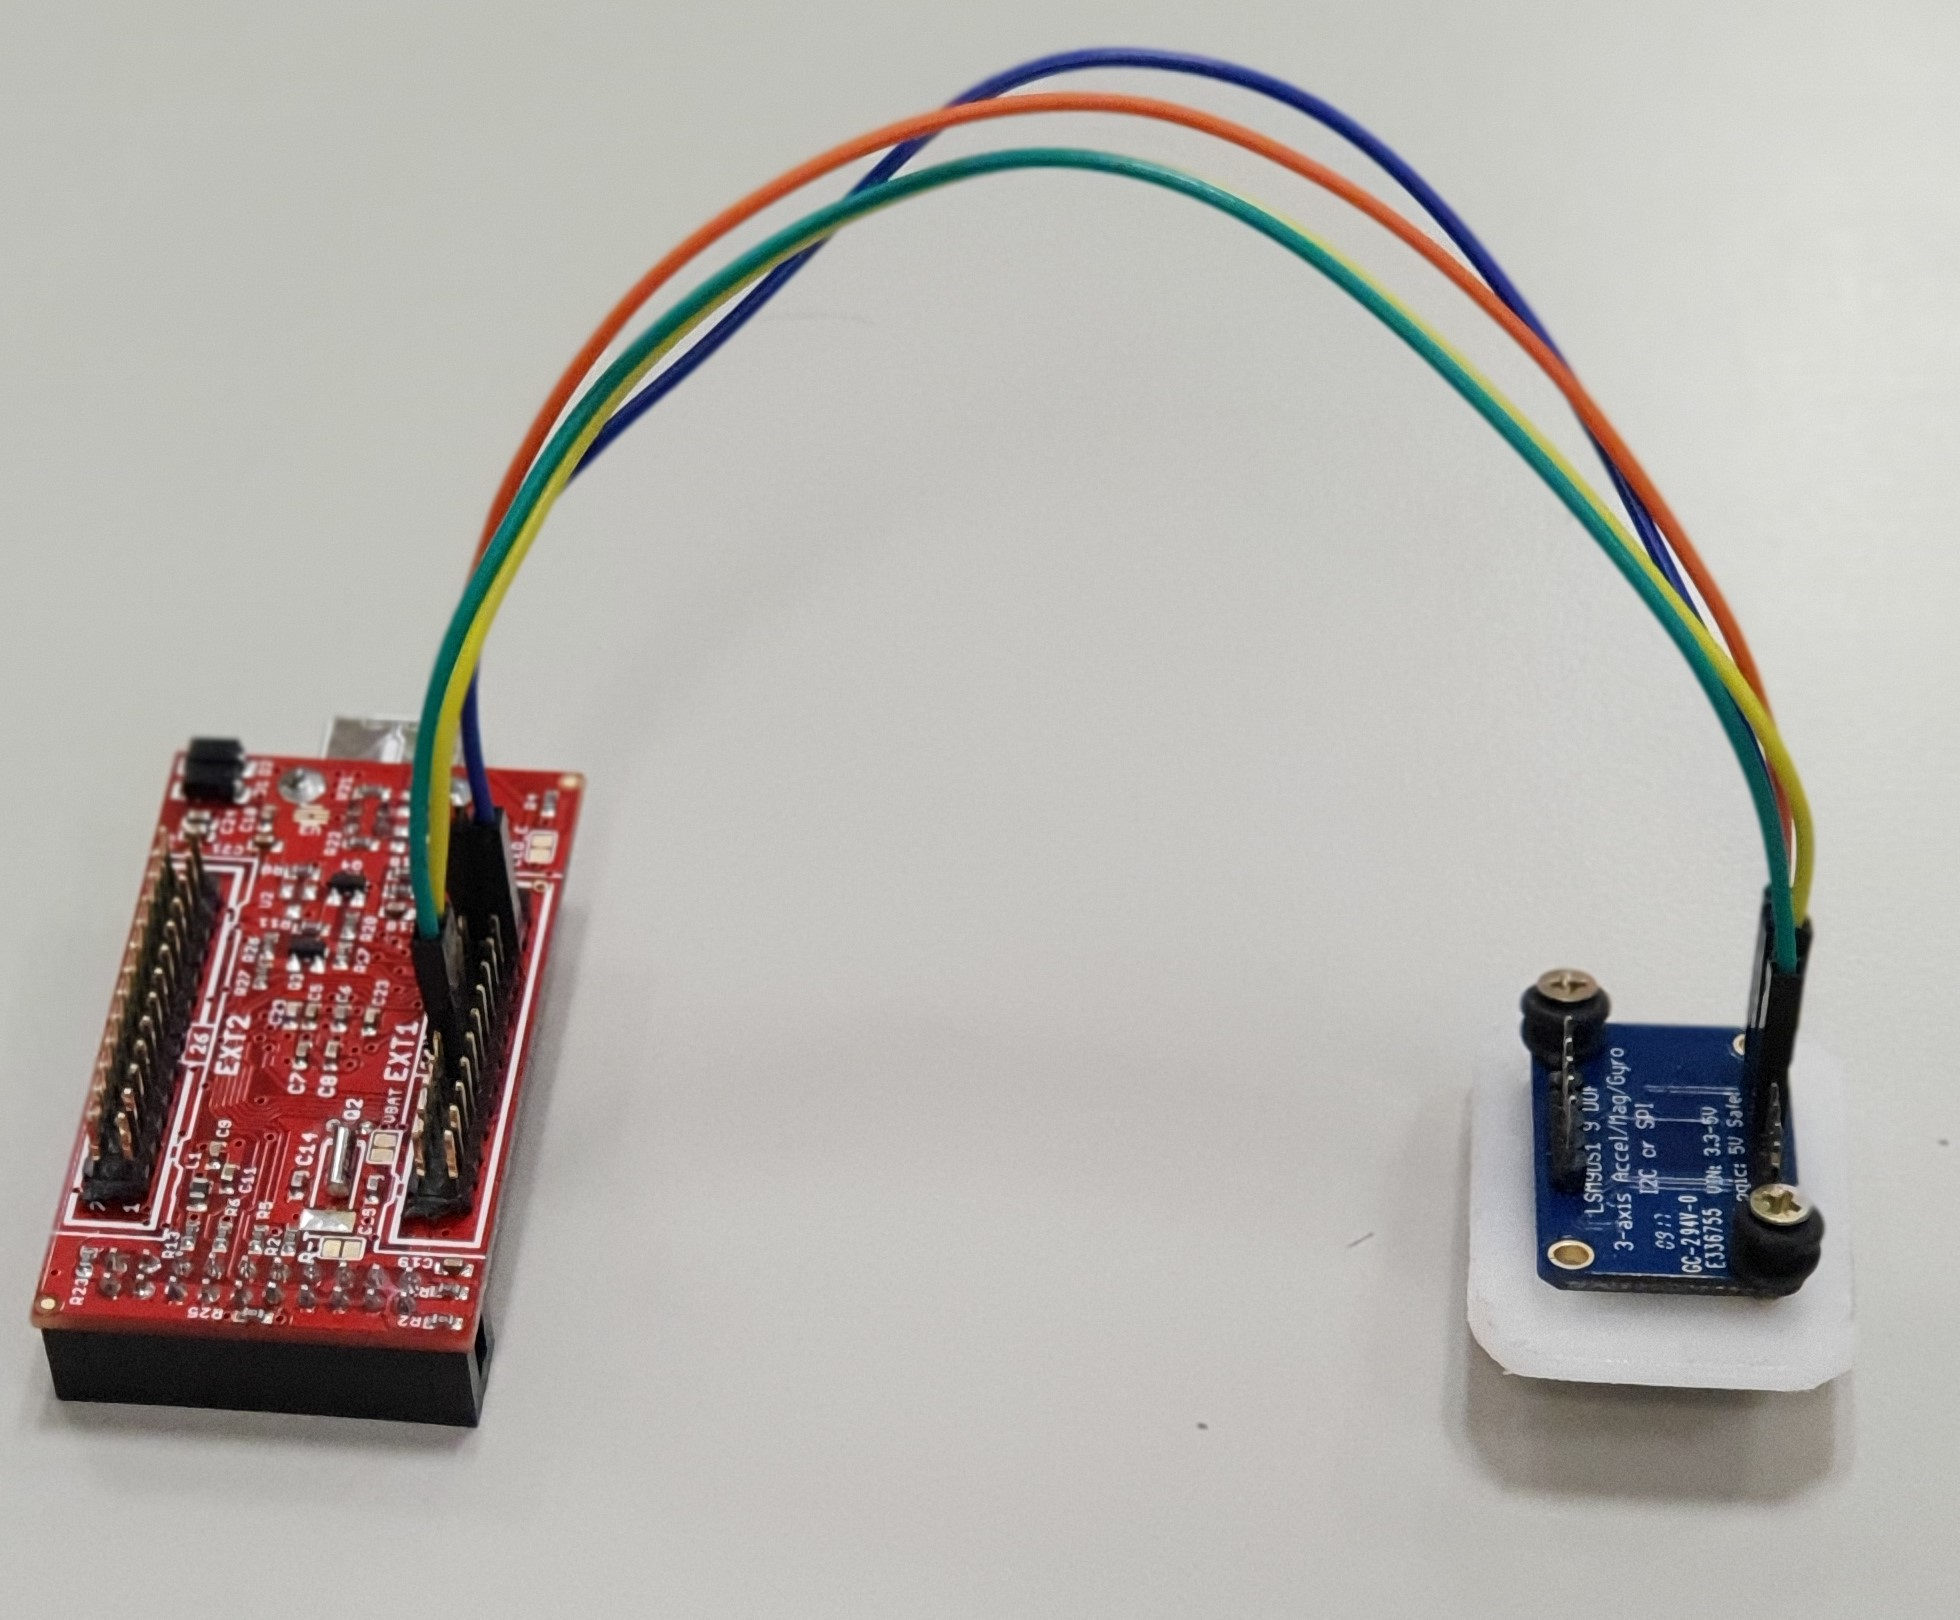
\includegraphics[scale=0.1]{implementazione/i2cFoto.jpg}
	\caption{Foto del canale di comunicazione I2C tra il microcontrollore e l'unità di misura inerziale.}
	\label{fig:i2cFoto}
\end{figure}
Il protocollo \cite{i2cWiki} dell'I2C richiede due linee seriali per comunicare correttamente:
\begin{itemize}
	\item SDA (\textit{Serial Data}) per i dati
	\item SCL (\textit{Serial Clock}) per sincronizzare i dispositivi
\end{itemize}
Vanno inoltre aggiunte una connessione di riferimento alla massa e una alla linea di alimentazione (tipicamente 5 o 3,3 V) a cui sono connessi resistori di \textit{pull-up}, come mostrato dalla figura seguente:
\begin{figure}[H]  
	\centering 
	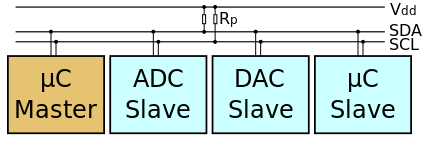
\includegraphics[scale=0.6]{implementazione/i2c.png}
	\caption{Rappresentazione di dispositivi collegati mediante I2C}
	\label{fig:i2c}
\end{figure}
L'I2C utilizza un indirizzo a 7 bit per un totale di 128 indirizzi disponibili. Poiché di questi 16 sono riservati, si ha un totale finale di 112 dispositivi collegabili alla medesima linea.\\
La velocità è il grande limite di questa comunicazione, infatti con le recenti revisioni si è riuscita a raggiungere una velocità massima di 3,4 Mbit/s (detto anche \textit{High Speed Mode}). Nello specifico di questa tesi lo si è utilizzato in \textit{fast mode} che corrisponde ad una velocità di 400 Kbit/s.\\
I dispositivi collegati al bus possono essere di due tipi:
\begin{itemize}
	\item Un \textit{Master} che controlla la SCL, inizializza le comunicazioni e invia dati
	\item Uno o più \textit{Slave} che rispondono ad un master e inviano dati
\end{itemize}

Il messaggio viene spezzato in due parti:
\begin{itemize}
	\item \textit{Address frame} dove il \textit{master} indica l'indirizzo dello \textit{slave} interessato alla comunicazione
	\item uno o più \textit{Data frames} contenenti l'informazione da trasmettere
\end{itemize}
I dati sono "piazzati" sulla linea SDA dopo che la linea SCL è posta a zero dal master, questi dati verranno letti dal dispositivo specificato nell'\textit{address frame} quando il \textit{master} riporterà la linea SCL al valore alto.\\
Relativamente al lavoro di questa tesi si identificano il \textit{Microcontrollore} come \textit{master} mentre l'\textit{IMU} come \textit{slave}. Nello specifico la comunicazione consiste nella lettura periodica da parte del microcontrollore dei valori misurati dai sensori all'interno dell'IMU. Tale lettura è stata realizzata leggendo i singoli registri ad 8 bit dei sensori (per maggiori dettagli si veda la stima temporale in sez.\ref{analisiTemporale}) attraverso lo script in Appendice \ref{scriptXLGRead} e rappresentato dalla seguente figura:
\begin{figure}[H]  
	\centering 
	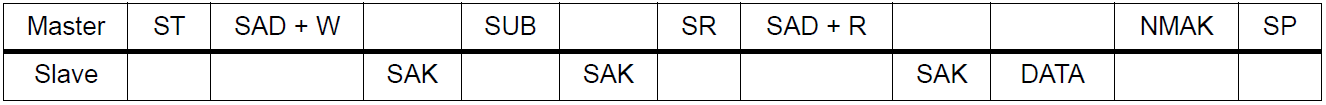
\includegraphics[scale=0.5]{implementazione/i2cRead.png}
	\caption{Rappresentazione del flusso di dati generato per la lettura, tramite I2C, di un registro ad 8 bit.}
	\label{fig:i2cRead}
\end{figure}
Dove:
\begin{itemize}
	\item  \textit{ST} è il segnale di inizio di una comunicazione
	\item \textit{SAD + W} include l'indirizzo del dispositivo slave mentre l'ultimo bit specifica che il master sta per scrivere
	\item \textit{SAK} lo slave con l'indirizzo specificato precedentemente risponde con un segnale di \textit{acknowledge}
	\item \textit{SUB} è l'indirizzo del registro interno del dispositivo specificato precedentemente
	\item \textit{SAK} lo slave risponde con un segnali di \textit{acknowledge} se l'indirizzo del registro esiste
	\item \textit{SR} è il bit di ripetizione dello start utilizzato in combinazione con SAD+R/W
	\item \textit{SAD + R} include l'indirizzo del dispositivo slave mentre l'ultimo bit specifica che il master vuole ricevere dati
	\item \textit{SAK} segnale di \textit{acknowledge} da parte dello \textit{slave}
	\item \textit{DATA} dati trasmetti nel formato ad 8 bit
	\item \textit{NMAK} segnale di  \textit{non acknowledge} da parte del \textit{master}
	\item \textit{SP} bit di stop della comunicazione
\end{itemize}
Tuttavia questa lettura non è sempre la migliore, infatti è possibile continuare a leggere i registri interni dello \textit{slave} trasmettendo il segnale di \textit{MAK} invece del segnale di \textit{NMAK} mostrato in Fig.\ref{fig:i2cRead}. In questo modo l'IMU incrementerà l'indirizzo del registro interno di partenza specificato in \textit{SUB} e provvederà a trasmettere il valore del registro interno successivo ad esso. Questa funzionalità è molto utile quando si devono leggere dati, come in questo caso, che sono rappresentati con più registri. Così facendo infatti si riduce l'\textit{overhead} della trasmissione e si migliora quindi il goodput generale rispetto alla lettura ripetuta dei singoli registri.\\



\subsubsection{USB CDC}
\label{imp_usbcdc}
Per la comunicazione tra il \textit{microcontrollore} e l'elaboratore si è utilizzato un canale di comunicazione USB nella classe CDC \cite{usbCDC}, mostrato in Fig.\ref{usbFoto}, attraverso la libreria \textit{HAL} \cite{hal} fornita da \textit{STM}.
\begin{figure}[H]  
	\centering 
	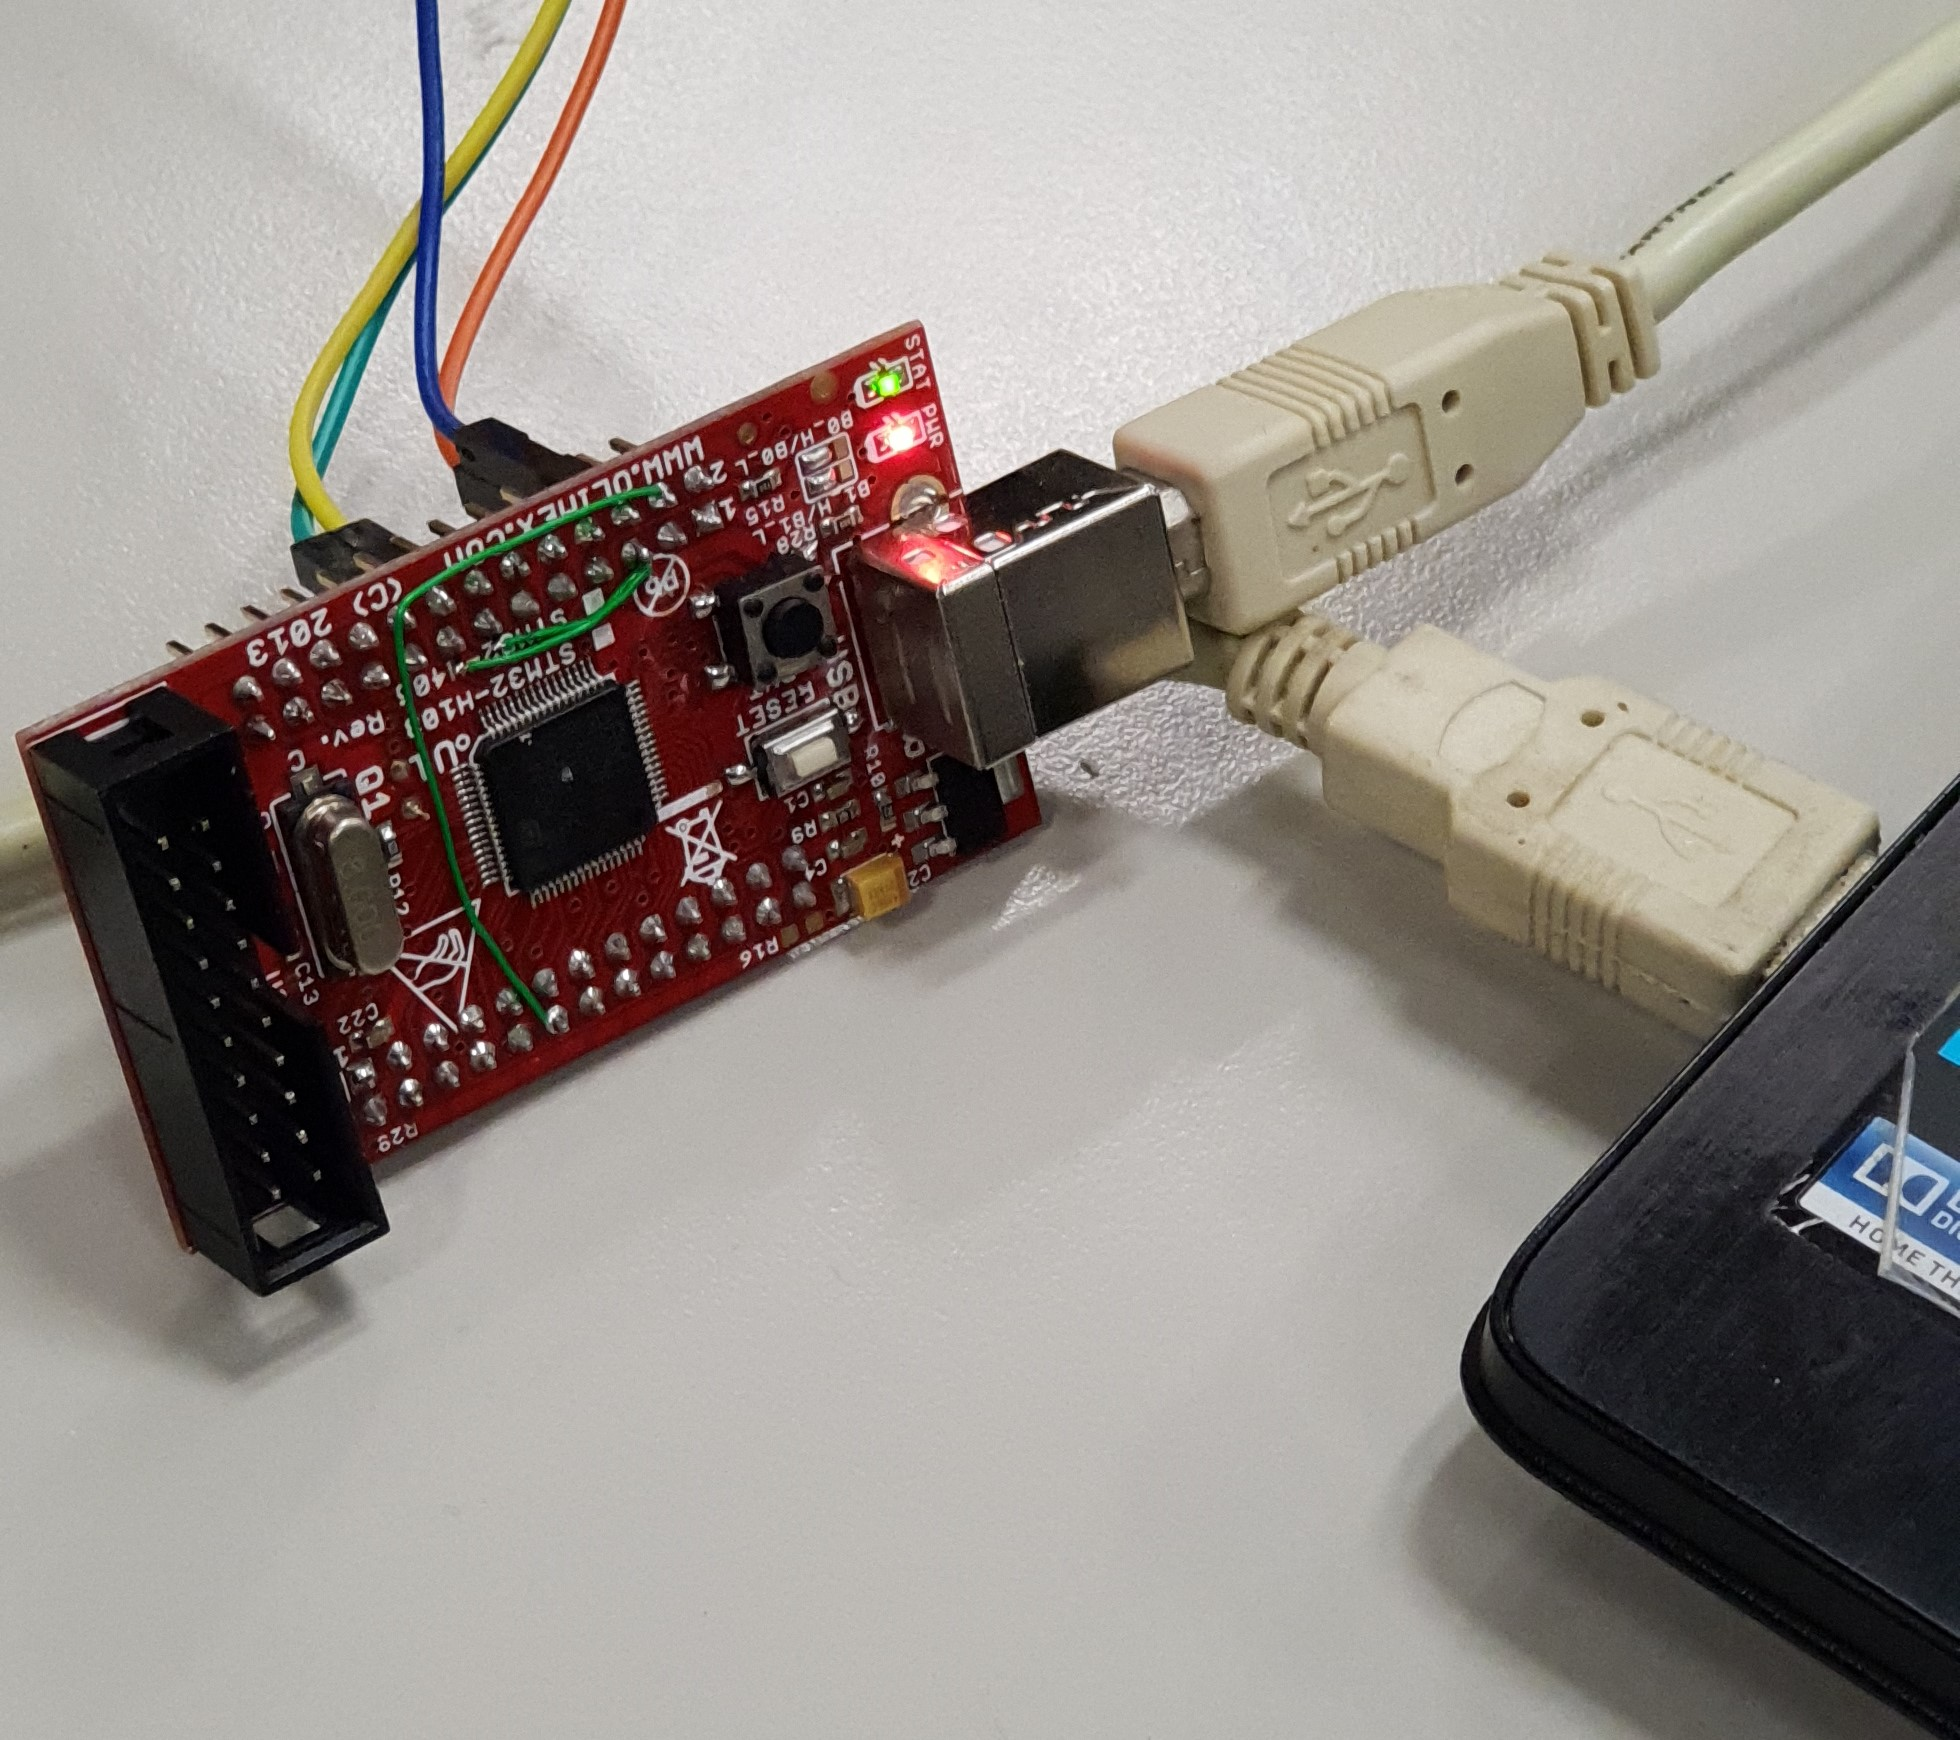
\includegraphics[scale=0.1]{implementazione/usbFoto.jpg}
	\caption{Foto del canale di comunicazione USB usato nella classe CDC per la trasmissione dei dati dal microcontrollore all'elaboratore.}
	\label{fig:usbFoto}
\end{figure}
Un dispositivo CDC è composto \cite{usbCDC2} dalle seguenti interfacce:
\begin{itemize}
	\item \textit{Communications Class Interface} (CCI)
	\item \textit{Data Class Interface} (DCI)
\end{itemize}
L'interfaccia CCI è responsabile della gestione del dispositivo e in alcuni casi anche della gestione delle chiamate. Per gestione del dispositivo si intendono le configurazioni necessarie da eseguire sul \textit{device} e la notifica degli eventi, mentre per gestione della chiamata si intendono le operazioni necessarie per stabilire e terminare una comunicazione. La CCI è obbligatoria per tutti i dispositivi CDC in quanto lo identifica specificando il modello di comunicazione supportato dal dispositivo stesso.\\
L'interfaccia DCI è responsabile della trasmissione dei dati, infatti i dati trasmessi e/o ricevuti non seguono uno specifico formato. Tutte le interfacce di questo tipo possono essere viste come interfacce subordinate della CCI.\\
Tutti i dispositivi CDC devono avere almeno un'interfaccia CCI e zero o più interfacce DCI. Un CCI e ogni suo DCI subordinato forniscono una specifica funzionalità al dispositivo.\\
In generale un \textit{device} CDC potrebbe supportare diverse funzionalità e quindi essere composto da diversi set di CCI e DCI, come mostrato dalla figura seguente:
\begin{figure}[H]  
	\centering 
	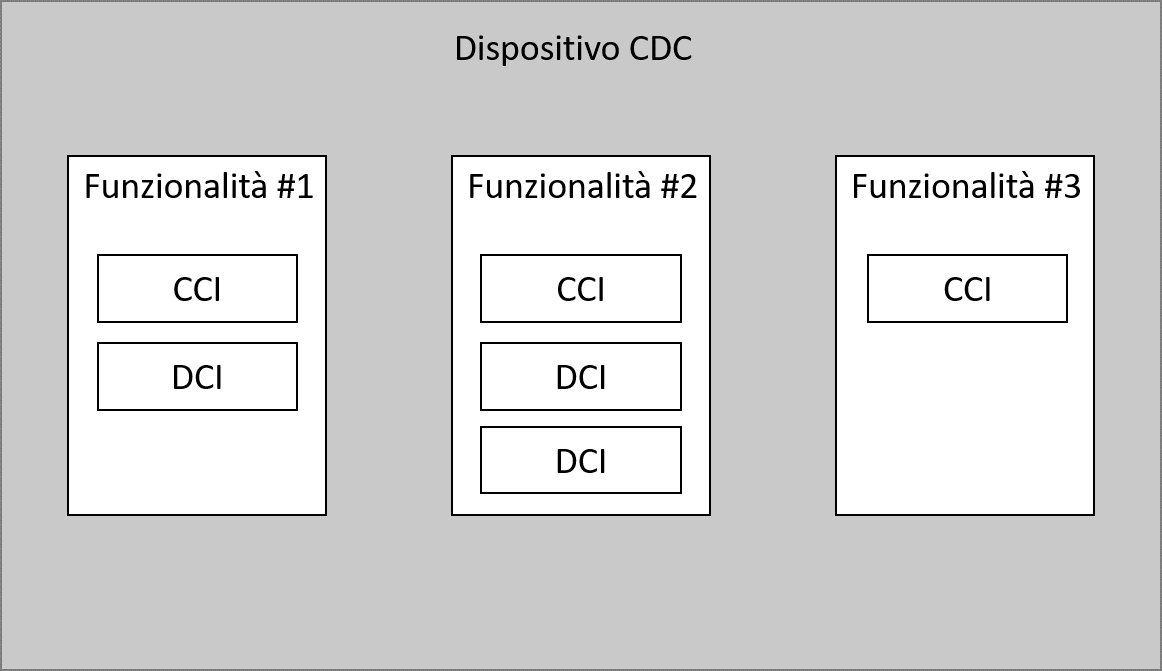
\includegraphics[scale=0.4]{implementazione/cdcDevice.png}
	\caption{Rappresentazione di un dispositivo CDC che supporta tre diverse funzionalità.}
	\label{fig:cdcDevice}
\end{figure}
Un dispositivo CDC solitamente usa le senguenti combinazioni di \textit{endpoints}:
\begin{itemize}
	\item Una coppia di \textit{endpoints} di controllo IN e OUT chiamate \textit{endpoint di default}.
	\item Un \textit{endpoint} opzionale chiamato \textit{bulk} o \textit{interrupt IN}
	\item Una coppia di \textit{bulk} o \textit{endpoints} IN e OUT asincroni
\end{itemize}
La tabella \ref{tab:endpoints} mostra gli usi dei differenti \textit{endpoints} sopracitati e da quale interfaccia sono utilizzati.
\begin{table}[H]
	\centering
	\label{tab:endpoints}
	\begin{tabular}{|c|c|c|c|}
		\hline
		\textbf{Endpoint}                          & \multicolumn{1}{l|}{\textbf{Direzione}}        & \multicolumn{1}{l|}{\textbf{Interfaccia}} & \textbf{Uso}                                                                                                                                                                   \\ \hline
		Control IN                                 & Device-\textgreater{}Host                      & CCI                                       & \begin{tabular}[c]{@{}c@{}}Richiesta standard \\ per l'enumerazione,\\ richiesta specifica della classe,\\ controllo del dispositivo e\\ controllo della chiamata\end{tabular} \\ \hline
		Control OUT                                & Host-\textgreater{}Device                      & CCI                                       & "..."                                                                                                                                                                          \\ \hline
		Interrupt o bulk IN                        & Device-\textgreater{}Host                      & CCI                                       & \begin{tabular}[c]{@{}c@{}}Notifica di un evento\\ come lo stato della linea \\ o della rete\end{tabular}                                                                      \\ \hline
		\multicolumn{1}{|l|}{Bulk o OUT asincrono} & \multicolumn{1}{l|}{Host-\textgreater{}Device} & DCI                                       & \begin{tabular}[c]{@{}c@{}}Comunicazione di \\ dati grezzi o formattati\end{tabular}                                                                                           \\ \hline
		Bulk o IN asincrono                        & Host-\textgreater{}Device                      & DCI                                       & "..."                                                                                                                                                                          \\ \hline
	\end{tabular}
	\caption{Tabella con gli usi tipici degli \textit{endpoints} per comunicazioni USB-CDC}
\end{table}
La libreria HAL utilizzata nel lavoro di questa tesi, utilizza due tipi di \textit{endpoints} per la comunicazione:
\begin{itemize}
	\item \textit{Endpoint Bulk} per il trasferimento dei dati (1 \textit{endpoint} di OUT e 1 \textit{endpoint} di IN)
	\item \textit{Endpoint interrupt} per il controllo della comunicazione (richieste CDC, 1 \textit{endpoint} IN)
\end{itemize}
Il trasferimento dei dati IN (dal \textit{device} verso l'\textit{host}) è gestito periodicamente in base alle richieste dell'\textit{host} (il \textit{device} specifica l'intervallo di tempo tra le richieste dei pacchetti). Per questo motivo, un buffer statico circolare viene usato per memorizzare i dati mandati dal terminale del \textit{device} (esempio USART nel caso di una \textit{Virtual COM Port}).\\
In generale, la comunicazione USB è molto più veloce dell'output del terminale (ad esempio il bitrate massimo di un USART è tipicamente 115 Kbps mentre il bitrate dell'USB 1.1 è 12 Mbps in \textit{Full speed mode} o 480 Mbps in \textit{High speed mode}). Di conseguenza, prima di mandare nuovi pacchetti l'\textit{host} deve aspettare finché il \textit{device} non termina di processare i dati precedentemente inviati. Quindi, nel caso di data OUT dall'\textit{host} verso il \textit{device} l'uso di un buffer statico circolare non avrebbe senso. Il driver sul \textit{device} aspetta che la procedura di processamento del dato precedente sia terminata prima di mandare un segnale di \textit{acknowledge} all'\textit{host}. \\
Infine la gestione delle richieste di controllo viene effettuata utilizzando o un \textit{endpoint} pari a zero oppure attraverso un \textit{endpoint interrupt} infatti se la dimensione del pacchetto di richiesta non eccede i 64 bytes, allora l'\textit{endpoint 0} è sufficiente a gestire tale richiesta. 






\section{Implementazione Software}
In questa sezione si mostrano alcuni dettagli riguardanti l'implementazione software. Nella parte iniziale si fornisce un \textit{overview} delle funzionalità dei due moduli (sez.\ref{livello_moduli}) mentre nell'ultima parte si mostrano le modalità operative identificate e realizzate.
\subsection{Diagramma Comportamentale}
Per una avere una visione generale delle funzionalità implementate nei moduli APP e microcontrollore, si mostrano due pseudo diagrammi di flusso che ne sintetizzano il comportamento di ciascuno dei due.
\subsubsection{Diagramma del Microcontrollore}
Il comportamento del modulo Microcontrollore può essere rappresentato mediante il seguente diagramma di flusso:
\begin{figure}[H]  
	\centering 
	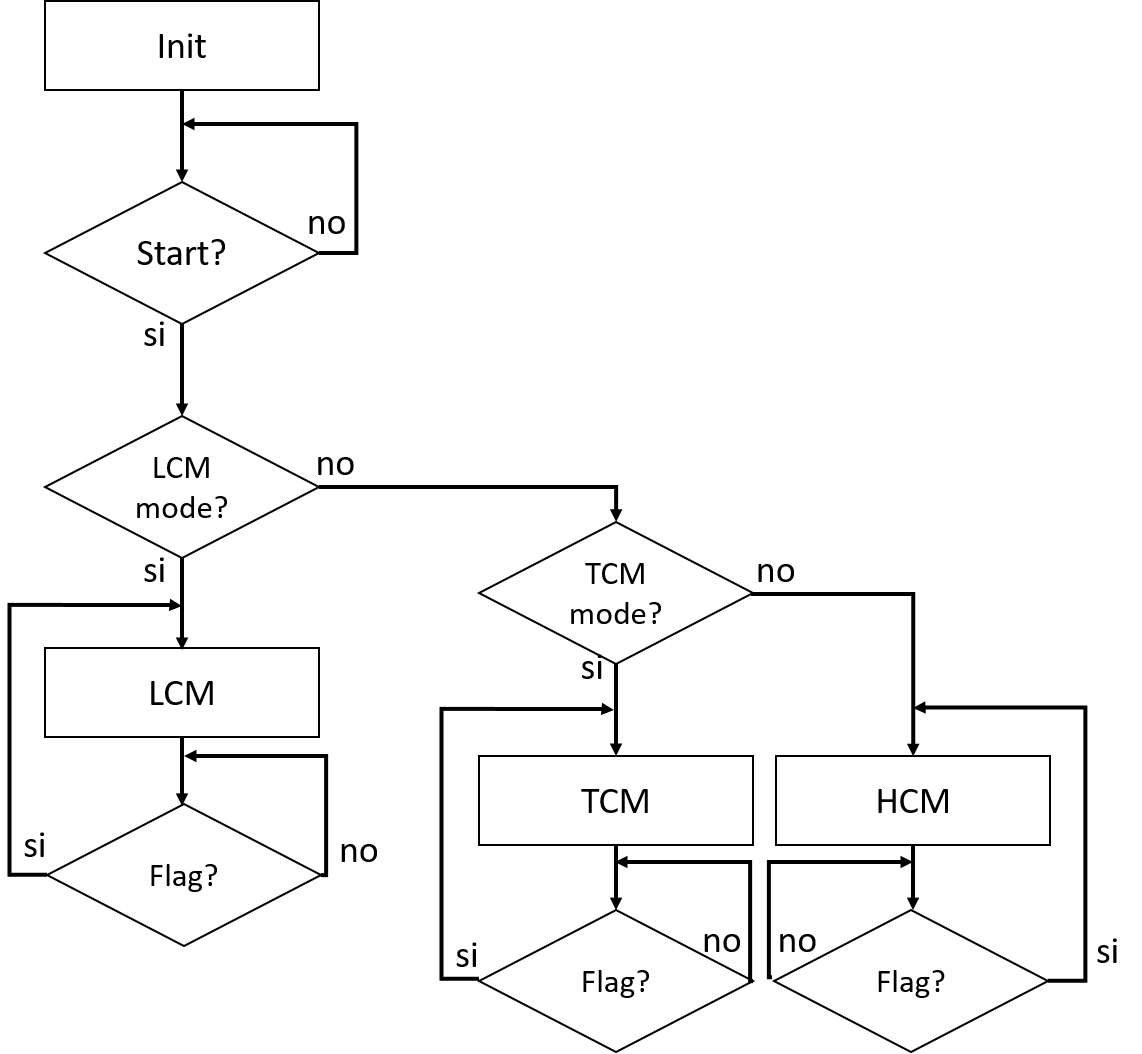
\includegraphics[scale=0.3]{implementazione/diagramma.png}
	\caption{Rappresentazione del comportamento per il modulo Microcontrollore.}
	\label{fig:diagrammaMicro}
\end{figure}
Dove:
\begin{itemize}
	\item \textbf{Init}: rappresenta la fase di inizializzazione del micro. L'utente sceglie la \textit{Computation Mode} e il numero di sensori da utilizzare (6DOF o 9DOF) modificando semplicemente due variabili globali (si veda appendice \ref{app:init}).
	\item \textbf{Start?}: il microcontrollore attende che il pulsante, integrato nella board, venga premuto di iniziare qualsiasi operazione.
	\item \textbf{LCM mode? e TCM mode?}: test di condizione sulla variabile globale che indica la \textit{Computation Mode} settata nella fase di inizializzazione. In base al suo valore il micro entrerà in un loop infinito della modalità scelta.
	\item \textbf{LCM}: procedura di \textit{Low Computation Mode}, sez.\ref{lcm}.
	\item \textbf{TCM}: procedura di \textit{Test Computation Mode}, sez.\ref{tcm}.
	\item \textbf{HCM}: procedura di \textit{High Computation Mode}, sez.\ref{hcm}.
	\item \textbf{Flag?}: test di condizione su una variabile di flag, modificata periodicamente da una routine tramite interrupt service.
\end{itemize}


\subsubsection{Diagramma del modulo APP}
Il comportamento del modulo APP relativo alla modalità \textbf{TCM} (sez.\ref{tcm}) può essere rappresentato mediante il seguente diagramma di flusso:
\begin{figure}[H]  
	\centering 
	\includegraphics[scale=0.4]{implementazione/diagrammaApp.png}
	\caption{Rappresentazione del comportamento per il modulo Microcontrollore.}
	\label{fig:diagrammaAPP}
\end{figure}
Dove:
\begin{itemize}
	\item \textbf{Init}: rappresenta la fase di inizializzazione della procedura. Vengono inizializzate le costanti necessarie all'algoritmo di sensor fusion (sez.\ref{sensor_fusion}), la variabile globale che definisce l'uso a 6DOF o 9DOF e infine i grafici da plottare successivamente.
	\item  \textbf{Read}: rappresenta la fase di lettura dei dati trasferiti dal modulo microcontrollore e salvati in un file di log. Ogni riga del file, corrispondente ad un pacchetto TCM (sez.\ref{tcm}), viene estratta e parsificata scomponendo la stringa in base ai separatori e i delimitatori utilizzati. Alla fine di questa fase si ottiene una matrice con i dati collezionati, per ogni sensore utilizzato, e una matrice con le stime dell'assetto elaborate dal microcontrollore.
	\item \textbf{Sensor Fusion}: rappresenta la fase di esecuzione dell'algoritmo di sensor fusion implementato (sez.\ref{descrizioneAlgoritmo}) a partire dalle matrici dei dati grezzi ottenuti nella fase precedente.
	\item \textbf{Plot stime}: vengono visualizzati gli angoli stimati dal microcontrollore e dal modulo APP al fine di completare l'analisi qualitativa dei due metodi (sez.\ref{analisiQualitativa})
\end{itemize}
Per i dettagli implementativi si rimanda alla lettura dell'Appendice \ref{app:tcmMatlab}.

\subsection{Modalità di computazione}
\label{computationMode}
In questa sezione verranno illustrate le modalità computazionali implementate all'interno del sistema (sez.\ref{livello_moduli}) e i relativi pacchetti dati utilizzati.

\subsubsection{Low Computation mode}
\label{lcm}
Questa modalità ha lo scopo di alleggerire il carico computazionale del microcontrollore, da qui il nome di \textit{low computation}. Infatti selezionandola l'algoritmo di \textit{sensor fusion}, per la stima dell'assetto (sez.\ref{sensor_fusion}), verrà eseguito dal modulo App, lasciando al microcontrollore la sola responsabilità di recuperare le misure effettuate dai sensori dell'IMU.\\
In questa modalità il pacchetto di dati da trasferire dal microcontrollore al modulo App ha la seguente struttura per la versione a 6DOF (giroscopio + accelerometro):
\begin{figure}[H]  
	\centering 
	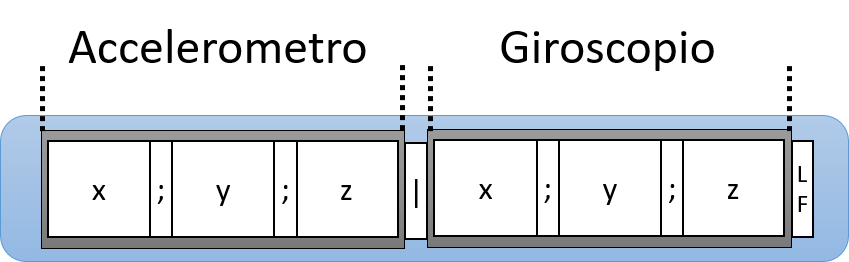
\includegraphics[scale=0.5]{implementazione/lcm6Foto.png}
	\caption{Rappresentazione del pacchetto dati utilizzato in \textit{Low Computation Mode} a 6DOF}
	\label{fig:lcm6Foto}
\end{figure}
Con riferimento alla Fig.\ref{fig:lcm6Foto}, si mostra la tabella riepilogativa dei singoli campi:
\begin{table}[H]
	\label{tab:packlcm6dof}
	\begin{tabular}{|c|c|c|c|}
		\hline
		\textbf{Campo}    & \textbf{\begin{tabular}[c]{@{}c@{}}Formattazione\\ dati\end{tabular}} & \textbf{\begin{tabular}[c]{@{}c@{}}Dimensione\\ (bytes)\end{tabular}} & \textbf{Descrizione}                                                                                            \\ \hline
		Accelerometro - X & x,xxx                                                                 & 5                                                                     & \begin{tabular}[c]{@{}c@{}}Accelerazione misurata \\ lungo l'asse X\end{tabular}                                \\ \hline
		Accelerometro - Y & y,yyy                                                                 & 5                                                                     & \begin{tabular}[c]{@{}c@{}}" " \\ lungo l'asse Y\end{tabular}                                 \\ \hline
		Accelerometro - Z & z,zzz                                                                 & 5                                                                     & \begin{tabular}[c]{@{}c@{}}" "\\ lungo l'asse Z\end{tabular}                                 \\ \hline
		$\mid$             & \multicolumn{1}{l|}{}                                                 & 1                                                                     & \begin{tabular}[c]{@{}c@{}}Delimitatore tra i dati \\ dell'accelerometro\\ e quelli del giroscopio\end{tabular} \\ \hline
		Giroscopio - X    & xxx,xxx                                                               & 7                                                                     & \begin{tabular}[c]{@{}c@{}}Velocità angolare\\ misurata attorno  all'asse X\end{tabular}                        \\ \hline
		Giroscopio - Y    & yyy,yyy                                                               & 7                                                                     & \begin{tabular}[c]{@{}c@{}}" "\\ misurata attorno  all'asse Y\end{tabular}                        \\ \hline
		Giroscopio - Z    & zzz,zzz                                                               & 7                                                                     & \begin{tabular}[c]{@{}c@{}}" "\\ misurata attorno  all'asse Z\end{tabular}                        \\ \hline
		LF                &                                                                       & 1                                                                     & \begin{tabular}[c]{@{}c@{}}Carattere ASCII per la \\ codifica del comando\\ "nuova riga"\end{tabular}           \\ \hline
	\end{tabular}
	\caption{Tabella riepilogativa dei campi presenti nel pacchetto dati in LCM a 6DOF}
\end{table}
A questi vanno aggiunti quattro campi ";"  utilizzati per separare le varie misure assiali dei sensori.\\
Sommando le dimensioni massime dei singoli campi mostrati in tab.\ref{tab:packlcm6dof} si ottiene facilmente che la dimensione massima del pacchetto dati nella modalità \textit{Low Computation} a 6DOF è di \textbf{42 bytes}.\\
Nell'uso a 9DOF viene aggiunto un campo per i dati provenienti dal magnetometro (sez.\ref{magnetometro}), ottenendo la seguente struttura:

\begin{figure}[H]  
	\centering 
	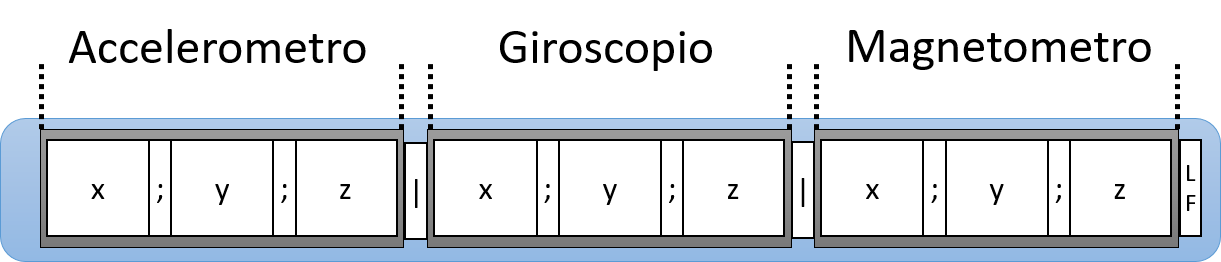
\includegraphics[scale=0.4]{implementazione/lcm9Foto.png}
	\caption{Rappresentazione del pacchetto dati utilizzato in \textit{Low Computation Mode} a 9DOF}
	\label{fig:lcm9Foto}
\end{figure}

Con riferimento alla Fig.\ref{fig:lcm9Foto}, si mostra la tabella riepilogativa dei singoli campi:

\begin{table}[H]
	\begin{tabular}{|c|c|c|c|}
		\hline
		\textbf{Campo}    & \textbf{\begin{tabular}[c]{@{}c@{}}Formattazione\\ dati\end{tabular}} & \textbf{\begin{tabular}[c]{@{}c@{}}Dimensione\\ (bytes)\end{tabular}} & \textbf{Descrizione}                                                                                  \\ \hline
		Accelerometro - X & x,xxx                                                                 & 5                                                                     & \begin{tabular}[c]{@{}c@{}}Accelerazione misurata \\ lungo l'asse X\end{tabular}                      \\ \hline
		Accelerometro - Y & y,yyy                                                                 & 5                                                                     & \begin{tabular}[c]{@{}c@{}}Accelerazione misurata\\ lungo l'asse Y\end{tabular}                       \\ \hline
		Accelerometro - Z & z,zzz                                                                 & 5                                                                     & \begin{tabular}[c]{@{}c@{}}Accelerazione misurata\\ lungo l'asse Z\end{tabular}                       \\ \hline
		$\mid$            & \multicolumn{1}{l|}{}                                                 & 1                                                                     & \begin{tabular}[c]{@{}c@{}}Delimitatore tra i dati \\ dei sensori\end{tabular}                        \\ \hline
		Giroscopio - X    & xxx,xxx                                                               & 7                                                                     & \begin{tabular}[c]{@{}c@{}}Velocità angolare\\ misurata attorno  all'asse X\end{tabular}              \\ \hline
		Giroscopio - Y    & yyy,yyy                                                               & 7                                                                     & \begin{tabular}[c]{@{}c@{}}Velocità angolare\\ misurata attorno  all'asse Y\end{tabular}              \\ \hline
		Giroscopio - Z    & zzz,zzz                                                               & 7                                                                     & \begin{tabular}[c]{@{}c@{}}Velocità angolare\\ misurata attorno  all'asse Z\end{tabular}              \\ \hline
		$\mid$            &                                                                       & 1                                                                     & \begin{tabular}[c]{@{}c@{}}Delimitatore tra i dati \\ dei sensori\end{tabular}                        \\ \hline
		Magnetometro- X   & x,xxx                                                                 & 5                                                                     & \begin{tabular}[c]{@{}c@{}}Intensità del campo\\ magnetico esterno\\ sull'asse X\end{tabular}         \\ \hline
		Magnetometro- Y   & y,yyy                                                                 & 5                                                                     & \begin{tabular}[c]{@{}c@{}}Intensità del campo\\ magnetico esterno\\ sull'asse Y\end{tabular}         \\ \hline
		Magnetometro- Z   & z,zzz                                                                 & 5                                                                     & \begin{tabular}[c]{@{}c@{}}Intensità del campo\\ magnetico esterno\\ sull'asse Z\end{tabular}         \\ \hline
		LF                &                                                                       & 1                                                                     & \begin{tabular}[c]{@{}c@{}}Carattere ASCII per la \\ codifica del comando\\ "nuova riga"\end{tabular} \\ \hline
	\end{tabular}
	\caption{Tabella riepilogativa dei campi presenti nel pacchetto dati in LCM a 9DOF}
\end{table}
Ancora una volta per determinare la dimensione totale del pacchetto, bisogna aggiungere i sei campi ";" che separano le varie misure assiali dei sensori. Così facendo si ottiene banalmente che la dimensione totale per la LCM in 9DOF è di \textbf{60 bytes}. Per i dettagli implementativi si rimanda alla lettura dell'appendice \ref{app:lcm}.

\subsubsection{High Computation mode}
\label{hcm}
Questa modalità permette di assegnare al microcontrollore anche il compito di stimare l'assetto utilizzando la libreria \textit{MotionFX} fornita da STM. Risulta evidente come questa modalità sia la duale della precedente (sez.\ref{lcm}) in quanto aumenta il carico computazionale del microcontrollore, da cui il nome \textit{High Computation}. \\
Analogamente a quanto fatto per la modalità LCM, si mostra la struttura del pacchetto da trasferire dal microcontrollore al modulo APP per questa modalità:

\begin{figure}[H]  
	\centering 
	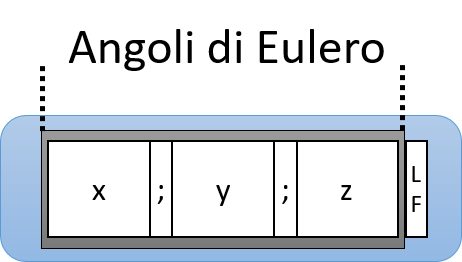
\includegraphics[scale=0.4]{implementazione/hcmFoto.png}
	\caption{Rappresentazione del pacchetto dati utilizzato in \textit{High Computation Mode}}
	\label{fig:hcmFoto}
\end{figure}
Si noti che in questo caso non vi sono distinzioni tra le strutture dei pacchetti a 6DOF e 9DOF, infatti indipendentemente da quanti sensori verranno utilizzati il microcontrollore dovrà sempre stimare l'assetto e mandarlo sotto forma di \textit{roll}, \textit{pitch} e \textit{yaw} (sez.\ref{angoliEulero}) al modulo APP. Con riferimento alla fig.\ref{fig:hcmFoto} si mostra la tabella riepilogativa dei campi:

\begin{table}[H]
	\centering
	\begin{tabular}{|c|c|c|c|}
		\hline
		\textbf{Campo} & \textbf{\begin{tabular}[c]{@{}c@{}}Formattazione\\ dati\end{tabular}} & \textbf{\begin{tabular}[c]{@{}c@{}}Dimensione\\ (bytes)\end{tabular}} & \textbf{Descrizione}                                                                                  \\ \hline
		Yaw            & xxx,x                                                                 & 5                                                                     &  \begin{tabular}[c]{@{}c@{}}Stima angolo\\ di imbardata\end{tabular}                                                               \\ \hline
		Pitch          & yyy,y                                                                 & 5                                                                     & \begin{tabular}[c]{@{}c@{}}Stima angolo\\ di beccheggio\end{tabular}                                            \\ \hline
		Roll           & zzz,z                                                                 & 5                                                                     & \begin{tabular}[c]{@{}c@{}}Stima angolo\\ di rollio\end{tabular}                                           \\ \hline
		LF             &                                                                       & 1                                                                     & \begin{tabular}[c]{@{}c@{}}Carattere ASCII per la \\ codifica del comando\\ "nuova riga"\end{tabular} \\ \hline
	\end{tabular}
\caption{Tabella riepilogativa dei campi presenti nel pacchetto dati in HCM}
\end{table}
Aggiungendo i due campi ";" utilizzati per separare gli angoli stimati, si ottiene che la dimensione del pacchetto dati da trasferire dal microcontrollore al modulo APP è di \textbf{18 bytes}.
Si noti come in questa modalità, pur aumentando il carico computazionale richiesto dal microcontrollore, si abbattano le dimensioni del pacchetto da trasferire al numero minimo di bytes necessari per rappresentare le stime degli angoli d'assetto in modo significativo. Per i dettagli implementativi si rimanda alla lettura dell'appendice \ref{app:hcm}.

\subsubsection{Testing Computation mode}
\label{tcm}
Quest'ultima modalità è stata pensata appositamente al fine di realizzare l'analisi qualitativa dell'assetto stimato (sez.\ref{analisiQualitativa}). La si può considerare come una modalità ibrida tra l'HCM e la LCM viste precedentemente, infatti in questo caso il pacchetto da trasferire dal microcontrollore al modulo APP include sia le misure dei sensori sia la stima dell'assetto.\\
In questa modalità il pacchetto di dati da trasferire dal microcontrollore al modulo App ha la seguente struttura per la versione a 6DOF:
\begin{figure}[H]  
	\centering 
	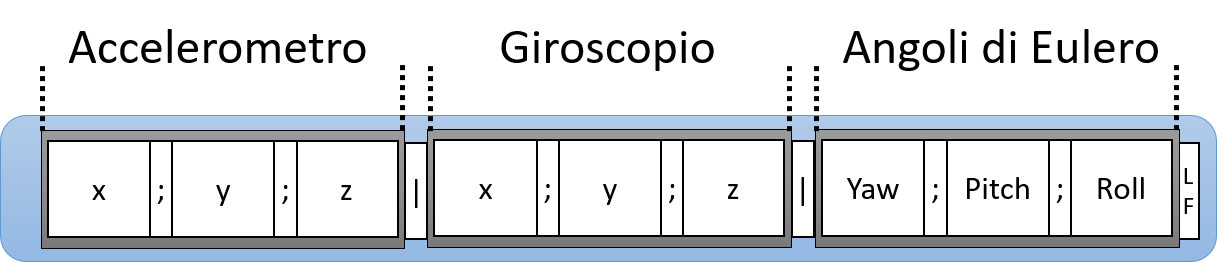
\includegraphics[scale=0.4]{implementazione/tcm6Foto.png}
	\caption{Rappresentazione del pacchetto dati utilizzato in \textit{Test Computation Mode} a 6DOF}
	\label{fig:tcm6Foto}
\end{figure}

Con riferimento alla Fig.\ref{fig:tcm6Foto}, si mostra la tabella riepilogativa dei singoli campi:
\begin{table}[H]
	\centering
	\begin{tabular}{|c|c|c|c|}
		\hline
		\textbf{Campo}    & \textbf{\begin{tabular}[c]{@{}c@{}}Formattazione\\ dati\end{tabular}} & \textbf{\begin{tabular}[c]{@{}c@{}}Dimensione\\ (bytes)\end{tabular}} & \textbf{Descrizione}                                                                                  \\ \hline
		Accelerometro - X & x,xxx                                                                 & 5                                                                     & \begin{tabular}[c]{@{}c@{}}Accelerazione misurata \\ lungo l'asse X\end{tabular}                      \\ \hline
		Accelerometro - Y & y,yyy                                                                 & 5                                                                     & \begin{tabular}[c]{@{}c@{}}Accelerazione misurata\\ lungo l'asse Y\end{tabular}                       \\ \hline
		Accelerometro - Z & z,zzz                                                                 & 5                                                                     & \begin{tabular}[c]{@{}c@{}}Accelerazione misurata\\ lungo l'asse Z\end{tabular}                       \\ \hline
		$\mid$            & \multicolumn{1}{l|}{}                                                 & 1                                                                     & \begin{tabular}[c]{@{}c@{}}Delimitatore tra i dati \\ dei sensori\end{tabular}                        \\ \hline
		Giroscopio - X    & xxx,xxx                                                               & 7                                                                     & \begin{tabular}[c]{@{}c@{}}Velocità angolare\\ misurata attorno  all'asse X\end{tabular}              \\ \hline
		Giroscopio - Y    & yyy,yyy                                                               & 7                                                                     & \begin{tabular}[c]{@{}c@{}}Velocità angolare\\ misurata attorno  all'asse Y\end{tabular}              \\ \hline
		Giroscopio - Z    & zzz,zzz                                                               & 7                                                                     & \begin{tabular}[c]{@{}c@{}}Velocità angolare\\ misurata attorno  all'asse Z\end{tabular}              \\ \hline
		$\mid$            &                                                                       & 1                                                                     & \begin{tabular}[c]{@{}c@{}}Delimitatore tra i dati \\ dei sensori\end{tabular}                        \\ \hline
		Yaw               & xxx,x                                                                 & 5                                                                     & \begin{tabular}[c]{@{}c@{}}Stima angolo\\ di imbardata\end{tabular}                                   \\ \hline
		Pitch             & yyy,y                                                                 & 5                                                                     & \begin{tabular}[c]{@{}c@{}}Stima angolo\\ di beccheggio\end{tabular}                                  \\ \hline
		Roll              & zzz,z                                                                 & 5                                                                     & \begin{tabular}[c]{@{}c@{}}Stima angolo\\ di rollio\end{tabular}                                      \\ \hline
		LF                &                                                                       & 1                                                                     & \begin{tabular}[c]{@{}c@{}}Carattere ASCII per la \\ codifica del comando\\ "nuova riga"\end{tabular} \\ \hline
	\end{tabular}
\caption{Tabella riepilogativa dei campi presenti nel pacchetto dati in TCM a 6DOF}
\end{table}
Ancora una volta aggiungendo sei campi ";" utilizzati per separare le misure assiali e gli angoli stimati si ottiene che la dimensione del pacchetto per questa modalità a 6DOF è  \textbf{60 bytes}.\\
Nell'uso a 9DOF viene aggiunto un campo per i dati provenienti dal magnetometro (sez.\ref{magnetometro}), ottenendo la seguente struttura:
\begin{figure}[H]  
	\centering 
	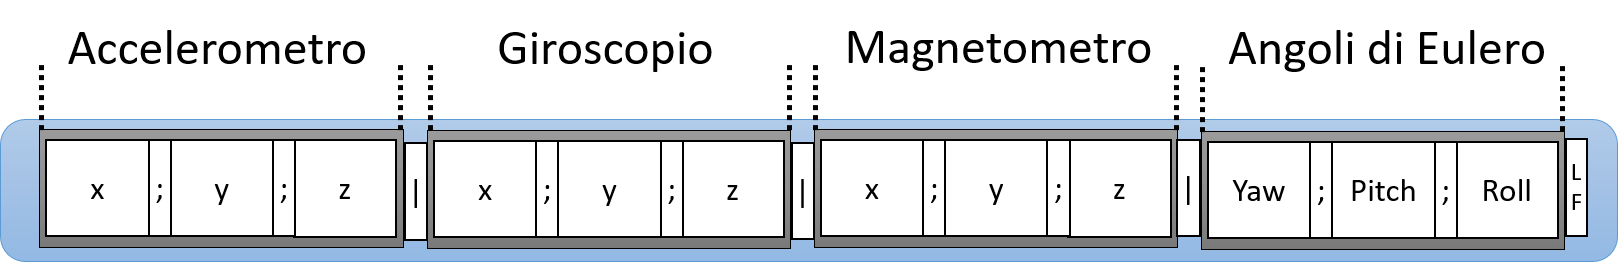
\includegraphics[scale=0.35]{implementazione/tcm9Foto.png}
	\caption{Rappresentazione del pacchetto dati utilizzato in \textit{Test Computation Mode} a 9DOF}
	\label{fig:tcm9Foto}
\end{figure}
Con riferimento alla Fig.\ref{fig:tcm9Foto}, si mostra la tabella riepilogativa dei singoli campi:

\begin{table}[H]
	\centering
	\begin{tabular}{|c|c|c|c|}
		\hline
		\textbf{Campo}    & \textbf{\begin{tabular}[c]{@{}c@{}}Formattazione\\ dati\end{tabular}} & \textbf{\begin{tabular}[c]{@{}c@{}}Dimensione\\ (bytes)\end{tabular}} & \textbf{Descrizione}                                                                                  \\ \hline
		Accelerometro - X & x,xxx                                                                 & 5                                                                     & \begin{tabular}[c]{@{}c@{}}Accelerazione misurata \\ lungo l'asse X\end{tabular}                      \\ \hline
		Accelerometro - Y & y,yyy                                                                 & 5                                                                     & \begin{tabular}[c]{@{}c@{}}Accelerazione misurata\\ lungo l'asse Y\end{tabular}                       \\ \hline
		Accelerometro - Z & z,zzz                                                                 & 5                                                                     & \begin{tabular}[c]{@{}c@{}}Accelerazione misurata\\ lungo l'asse Z\end{tabular}                       \\ \hline
		$\mid$            & \multicolumn{1}{l|}{}                                                 & 1                                                                     & \begin{tabular}[c]{@{}c@{}}Delimitatore tra i dati \\ dei sensori\end{tabular}                        \\ \hline
		Giroscopio - X    & xxx,xxx                                                               & 7                                                                     & \begin{tabular}[c]{@{}c@{}}Velocità angolare\\ misurata attorno  all'asse X\end{tabular}              \\ \hline
		Giroscopio - Y    & yyy,yyy                                                               & 7                                                                     & \begin{tabular}[c]{@{}c@{}}Velocità angolare\\ misurata attorno  all'asse Y\end{tabular}              \\ \hline
		Giroscopio - Z    & zzz,zzz                                                               & 7                                                                     & \begin{tabular}[c]{@{}c@{}}Velocità angolare\\ misurata attorno  all'asse Z\end{tabular}              \\ \hline
		$\mid$            &                                                                       & 1                                                                     & \begin{tabular}[c]{@{}c@{}}Delimitatore tra i dati \\ dei sensori\end{tabular}                        \\ \hline
		Magnetometro- X   & x,xxx                                                                 & 5                                                                     & \begin{tabular}[c]{@{}c@{}}Intensità del campo\\ magnetico esterno\\ sull'asse X\end{tabular}         \\ \hline
		Magnetometro- Y   & y,yyy                                                                 & 5                                                                     & \begin{tabular}[c]{@{}c@{}}Intensità del campo\\ magnetico esterno\\ sull'asse Y\end{tabular}         \\ \hline
		Magnetometro- Z   & z,zzz                                                                 & 5                                                                     & \begin{tabular}[c]{@{}c@{}}Intensità del campo\\ magnetico esterno\\ sull'asse Z\end{tabular}         \\ \hline
		$\mid$            &                                                                       & 1                                                                     & \begin{tabular}[c]{@{}c@{}}Delimitatore tra i\\ dati dei sensori e\\ l'assetto stimato\end{tabular}   \\ \hline
		Yaw               & xxx,x                                                                 & 5                                                                     & \begin{tabular}[c]{@{}c@{}}Stima angolo\\ di imbardata\end{tabular}                                   \\ \hline
		Pitch             & yyy,y                                                                 & 5                                                                     & \begin{tabular}[c]{@{}c@{}}Stima angolo\\ di beccheggio\end{tabular}                                  \\ \hline
		Roll              & zzz,z                                                                 & 5                                                                     & \begin{tabular}[c]{@{}c@{}}Stima angolo\\ di rollio\end{tabular}                                      \\ \hline
		LF                &                                                                       & 1                                                                     & \begin{tabular}[c]{@{}c@{}}Carattere ASCII per la \\ codifica del comando\\ "nuova riga"\end{tabular} \\ \hline
	\end{tabular}
\caption{Tabella riepilogativa dei campi presenti nel pacchetto dati in TCM a 9DOF}
\end{table}
Infine aggiungendo otto campi ";" utilizzati per separare le misure assiali e gli angoli stimati si ottiene che la dimensione del pacchetto per questa modalità a 9DOF è  \textbf{78 bytes}.\\
Quindi la TCM a 9DOF risulta essere la modalità con il maggiore carico computazionale richiesto al microcontrollore e con la dimensione maggiore dei pacchetti da trasferire dal micro al modulo APP. Per i dettagli implementativi si rimanda alla lettura dell'appendice \ref{app:tcm}.

